\documentclass[twoside]{book}

% Packages required by doxygen
\usepackage{calc}
\usepackage{doxygen}
\usepackage{graphicx}
\usepackage[utf8]{inputenc}
\usepackage{makeidx}
\usepackage{multicol}
\usepackage{multirow}
\usepackage{textcomp}
\usepackage[table]{xcolor}

% Font selection
\usepackage[T1]{fontenc}
\usepackage{mathptmx}
\usepackage[scaled=.90]{helvet}
\usepackage{courier}
\usepackage{amssymb}
\usepackage{sectsty}
\renewcommand{\familydefault}{\sfdefault}
\allsectionsfont{%
  \fontseries{bc}\selectfont%
  \color{darkgray}%
}
\renewcommand{\DoxyLabelFont}{%
  \fontseries{bc}\selectfont%
  \color{darkgray}%
}

% Page & text layout
\usepackage{geometry}
\geometry{%
  a4paper,%
  top=2.5cm,%
  bottom=2.5cm,%
  left=2.5cm,%
  right=2.5cm%
}
\tolerance=750
\hfuzz=15pt
\hbadness=750
\setlength{\emergencystretch}{15pt}
\setlength{\parindent}{0cm}
\setlength{\parskip}{0.2cm}
\makeatletter
\renewcommand{\paragraph}{%
  \@startsection{paragraph}{4}{0ex}{-1.0ex}{1.0ex}{%
    \normalfont\normalsize\bfseries\SS@parafont%
  }%
}
\renewcommand{\subparagraph}{%
  \@startsection{subparagraph}{5}{0ex}{-1.0ex}{1.0ex}{%
    \normalfont\normalsize\bfseries\SS@subparafont%
  }%
}
\makeatother

% Headers & footers
\usepackage{fancyhdr}
\pagestyle{fancyplain}
\fancyhead[LE]{\fancyplain{}{\bfseries\thepage}}
\fancyhead[CE]{\fancyplain{}{}}
\fancyhead[RE]{\fancyplain{}{\bfseries\leftmark}}
\fancyhead[LO]{\fancyplain{}{\bfseries\rightmark}}
\fancyhead[CO]{\fancyplain{}{}}
\fancyhead[RO]{\fancyplain{}{\bfseries\thepage}}
\fancyfoot[LE]{\fancyplain{}{}}
\fancyfoot[CE]{\fancyplain{}{}}
\fancyfoot[RE]{\fancyplain{}{\bfseries\scriptsize Generated on Mon Jun 2 2014 01:42:09 for My Project by Doxygen }}
\fancyfoot[LO]{\fancyplain{}{\bfseries\scriptsize Generated on Mon Jun 2 2014 01:42:09 for My Project by Doxygen }}
\fancyfoot[CO]{\fancyplain{}{}}
\fancyfoot[RO]{\fancyplain{}{}}
\renewcommand{\footrulewidth}{0.4pt}
\renewcommand{\chaptermark}[1]{%
  \markboth{#1}{}%
}
\renewcommand{\sectionmark}[1]{%
  \markright{\thesection\ #1}%
}

% Indices & bibliography
\usepackage{natbib}
\usepackage[titles]{tocloft}
\setcounter{tocdepth}{3}
\setcounter{secnumdepth}{5}
\makeindex

% Hyperlinks (required, but should be loaded last)
\usepackage{ifpdf}
\ifpdf
  \usepackage[pdftex,pagebackref=true]{hyperref}
\else
  \usepackage[ps2pdf,pagebackref=true]{hyperref}
\fi
\hypersetup{%
  colorlinks=true,%
  linkcolor=blue,%
  citecolor=blue,%
  unicode%
}

% Custom commands
\newcommand{\clearemptydoublepage}{%
  \newpage{\pagestyle{empty}\cleardoublepage}%
}


%===== C O N T E N T S =====

\begin{document}

% Titlepage & ToC
\hypersetup{pageanchor=false}
\pagenumbering{roman}
\begin{titlepage}
\vspace*{7cm}
\begin{center}%
{\Large My Project }\\
\vspace*{1cm}
{\large Generated by Doxygen 1.8.4}\\
\vspace*{0.5cm}
{\small Mon Jun 2 2014 01:42:09}\\
\end{center}
\end{titlepage}
\clearemptydoublepage
\tableofcontents
\clearemptydoublepage
\pagenumbering{arabic}
\hypersetup{pageanchor=true}

%--- Begin generated contents ---
\chapter{File Index}
\section{File List}
Here is a list of all files with brief descriptions\-:\begin{DoxyCompactList}
\item\contentsline{section}{/home/guille/msm/net/mac80211/\hyperlink{aes__ccm_8c}{aes\-\_\-ccm.\-c} }{\pageref{aes__ccm_8c}}{}
\item\contentsline{section}{/home/guille/msm/net/mac80211/\hyperlink{aes__ccm_8h}{aes\-\_\-ccm.\-h} }{\pageref{aes__ccm_8h}}{}
\item\contentsline{section}{/home/guille/msm/net/mac80211/\hyperlink{aes__cmac_8c}{aes\-\_\-cmac.\-c} }{\pageref{aes__cmac_8c}}{}
\item\contentsline{section}{/home/guille/msm/net/mac80211/\hyperlink{aes__cmac_8h}{aes\-\_\-cmac.\-h} }{\pageref{aes__cmac_8h}}{}
\item\contentsline{section}{/home/guille/msm/net/mac80211/\hyperlink{agg-rx_8c}{agg-\/rx.\-c} }{\pageref{agg-rx_8c}}{}
\item\contentsline{section}{/home/guille/msm/net/mac80211/\hyperlink{agg-tx_8c}{agg-\/tx.\-c} }{\pageref{agg-tx_8c}}{}
\item\contentsline{section}{/home/guille/msm/net/mac80211/\hyperlink{cfg_8c}{cfg.\-c} }{\pageref{cfg_8c}}{}
\item\contentsline{section}{/home/guille/msm/net/mac80211/\hyperlink{cfg_8h}{cfg.\-h} }{\pageref{cfg_8h}}{}
\item\contentsline{section}{/home/guille/msm/net/mac80211/\hyperlink{chan_8c}{chan.\-c} }{\pageref{chan_8c}}{}
\item\contentsline{section}{/home/guille/msm/net/mac80211/\hyperlink{debugfs_8c}{debugfs.\-c} }{\pageref{debugfs_8c}}{}
\item\contentsline{section}{/home/guille/msm/net/mac80211/\hyperlink{debugfs_8h}{debugfs.\-h} }{\pageref{debugfs_8h}}{}
\item\contentsline{section}{/home/guille/msm/net/mac80211/\hyperlink{debugfs__key_8c}{debugfs\-\_\-key.\-c} }{\pageref{debugfs__key_8c}}{}
\item\contentsline{section}{/home/guille/msm/net/mac80211/\hyperlink{debugfs__key_8h}{debugfs\-\_\-key.\-h} }{\pageref{debugfs__key_8h}}{}
\item\contentsline{section}{/home/guille/msm/net/mac80211/\hyperlink{debugfs__netdev_8c}{debugfs\-\_\-netdev.\-c} }{\pageref{debugfs__netdev_8c}}{}
\item\contentsline{section}{/home/guille/msm/net/mac80211/\hyperlink{debugfs__netdev_8h}{debugfs\-\_\-netdev.\-h} }{\pageref{debugfs__netdev_8h}}{}
\item\contentsline{section}{/home/guille/msm/net/mac80211/\hyperlink{debugfs__sta_8c}{debugfs\-\_\-sta.\-c} }{\pageref{debugfs__sta_8c}}{}
\item\contentsline{section}{/home/guille/msm/net/mac80211/\hyperlink{debugfs__sta_8h}{debugfs\-\_\-sta.\-h} }{\pageref{debugfs__sta_8h}}{}
\item\contentsline{section}{/home/guille/msm/net/mac80211/\hyperlink{driver-ops_8h}{driver-\/ops.\-h} }{\pageref{driver-ops_8h}}{}
\item\contentsline{section}{/home/guille/msm/net/mac80211/\hyperlink{driver-trace_8c}{driver-\/trace.\-c} }{\pageref{driver-trace_8c}}{}
\item\contentsline{section}{/home/guille/msm/net/mac80211/\hyperlink{driver-trace_8h}{driver-\/trace.\-h} }{\pageref{driver-trace_8h}}{}
\item\contentsline{section}{/home/guille/msm/net/mac80211/\hyperlink{event_8c}{event.\-c} }{\pageref{event_8c}}{}
\item\contentsline{section}{/home/guille/msm/net/mac80211/\hyperlink{ht_8c}{ht.\-c} }{\pageref{ht_8c}}{}
\item\contentsline{section}{/home/guille/msm/net/mac80211/\hyperlink{ibss_8c}{ibss.\-c} }{\pageref{ibss_8c}}{}
\item\contentsline{section}{/home/guille/msm/net/mac80211/\hyperlink{ieee80211__i_8h}{ieee80211\-\_\-i.\-h} }{\pageref{ieee80211__i_8h}}{}
\item\contentsline{section}{/home/guille/msm/net/mac80211/\hyperlink{iface_8c}{iface.\-c} }{\pageref{iface_8c}}{}
\item\contentsline{section}{/home/guille/msm/net/mac80211/\hyperlink{key_8c}{key.\-c} }{\pageref{key_8c}}{}
\item\contentsline{section}{/home/guille/msm/net/mac80211/\hyperlink{key_8h}{key.\-h} }{\pageref{key_8h}}{}
\item\contentsline{section}{/home/guille/msm/net/mac80211/\hyperlink{led_8c}{led.\-c} }{\pageref{led_8c}}{}
\item\contentsline{section}{/home/guille/msm/net/mac80211/\hyperlink{led_8h}{led.\-h} }{\pageref{led_8h}}{}
\item\contentsline{section}{/home/guille/msm/net/mac80211/\hyperlink{main_8c}{main.\-c} }{\pageref{main_8c}}{}
\item\contentsline{section}{/home/guille/msm/net/mac80211/\hyperlink{mesh_8c}{mesh.\-c} }{\pageref{mesh_8c}}{}
\item\contentsline{section}{/home/guille/msm/net/mac80211/\hyperlink{mesh_8h}{mesh.\-h} }{\pageref{mesh_8h}}{}
\item\contentsline{section}{/home/guille/msm/net/mac80211/\hyperlink{mesh__hwmp_8c}{mesh\-\_\-hwmp.\-c} }{\pageref{mesh__hwmp_8c}}{}
\item\contentsline{section}{/home/guille/msm/net/mac80211/\hyperlink{mesh__pathtbl_8c}{mesh\-\_\-pathtbl.\-c} }{\pageref{mesh__pathtbl_8c}}{}
\item\contentsline{section}{/home/guille/msm/net/mac80211/\hyperlink{mesh__plink_8c}{mesh\-\_\-plink.\-c} }{\pageref{mesh__plink_8c}}{}
\item\contentsline{section}{/home/guille/msm/net/mac80211/\hyperlink{michael_8c}{michael.\-c} }{\pageref{michael_8c}}{}
\item\contentsline{section}{/home/guille/msm/net/mac80211/\hyperlink{michael_8h}{michael.\-h} }{\pageref{michael_8h}}{}
\item\contentsline{section}{/home/guille/msm/net/mac80211/\hyperlink{mlme_8c}{mlme.\-c} }{\pageref{mlme_8c}}{}
\item\contentsline{section}{/home/guille/msm/net/mac80211/\hyperlink{offchannel_8c}{offchannel.\-c} }{\pageref{offchannel_8c}}{}
\item\contentsline{section}{/home/guille/msm/net/mac80211/\hyperlink{pm_8c}{pm.\-c} }{\pageref{pm_8c}}{}
\item\contentsline{section}{/home/guille/msm/net/mac80211/\hyperlink{rate_8c}{rate.\-c} }{\pageref{rate_8c}}{}
\item\contentsline{section}{/home/guille/msm/net/mac80211/\hyperlink{rate_8h}{rate.\-h} }{\pageref{rate_8h}}{}
\item\contentsline{section}{/home/guille/msm/net/mac80211/\hyperlink{rc80211__minstrel_8c}{rc80211\-\_\-minstrel.\-c} }{\pageref{rc80211__minstrel_8c}}{}
\item\contentsline{section}{/home/guille/msm/net/mac80211/\hyperlink{rc80211__minstrel_8h}{rc80211\-\_\-minstrel.\-h} }{\pageref{rc80211__minstrel_8h}}{}
\item\contentsline{section}{/home/guille/msm/net/mac80211/\hyperlink{rc80211__minstrel__debugfs_8c}{rc80211\-\_\-minstrel\-\_\-debugfs.\-c} }{\pageref{rc80211__minstrel__debugfs_8c}}{}
\item\contentsline{section}{/home/guille/msm/net/mac80211/\hyperlink{rc80211__minstrel__ht_8c}{rc80211\-\_\-minstrel\-\_\-ht.\-c} }{\pageref{rc80211__minstrel__ht_8c}}{}
\item\contentsline{section}{/home/guille/msm/net/mac80211/\hyperlink{rc80211__minstrel__ht_8h}{rc80211\-\_\-minstrel\-\_\-ht.\-h} }{\pageref{rc80211__minstrel__ht_8h}}{}
\item\contentsline{section}{/home/guille/msm/net/mac80211/\hyperlink{rc80211__minstrel__ht__debugfs_8c}{rc80211\-\_\-minstrel\-\_\-ht\-\_\-debugfs.\-c} }{\pageref{rc80211__minstrel__ht__debugfs_8c}}{}
\item\contentsline{section}{/home/guille/msm/net/mac80211/\hyperlink{rc80211__pid_8h}{rc80211\-\_\-pid.\-h} }{\pageref{rc80211__pid_8h}}{}
\item\contentsline{section}{/home/guille/msm/net/mac80211/\hyperlink{rc80211__pid__algo_8c}{rc80211\-\_\-pid\-\_\-algo.\-c} }{\pageref{rc80211__pid__algo_8c}}{}
\item\contentsline{section}{/home/guille/msm/net/mac80211/\hyperlink{rc80211__pid__debugfs_8c}{rc80211\-\_\-pid\-\_\-debugfs.\-c} }{\pageref{rc80211__pid__debugfs_8c}}{}
\item\contentsline{section}{/home/guille/msm/net/mac80211/\hyperlink{rx_8c}{rx.\-c} }{\pageref{rx_8c}}{}
\item\contentsline{section}{/home/guille/msm/net/mac80211/\hyperlink{scan_8c}{scan.\-c} }{\pageref{scan_8c}}{}
\item\contentsline{section}{/home/guille/msm/net/mac80211/\hyperlink{spectmgmt_8c}{spectmgmt.\-c} }{\pageref{spectmgmt_8c}}{}
\item\contentsline{section}{/home/guille/msm/net/mac80211/\hyperlink{sta__info_8c}{sta\-\_\-info.\-c} }{\pageref{sta__info_8c}}{}
\item\contentsline{section}{/home/guille/msm/net/mac80211/\hyperlink{sta__info_8h}{sta\-\_\-info.\-h} }{\pageref{sta__info_8h}}{}
\item\contentsline{section}{/home/guille/msm/net/mac80211/\hyperlink{status_8c}{status.\-c} }{\pageref{status_8c}}{}
\item\contentsline{section}{/home/guille/msm/net/mac80211/\hyperlink{tkip_8c}{tkip.\-c} }{\pageref{tkip_8c}}{}
\item\contentsline{section}{/home/guille/msm/net/mac80211/\hyperlink{tkip_8h}{tkip.\-h} }{\pageref{tkip_8h}}{}
\item\contentsline{section}{/home/guille/msm/net/mac80211/\hyperlink{tx_8c}{tx.\-c} }{\pageref{tx_8c}}{}
\item\contentsline{section}{/home/guille/msm/net/mac80211/\hyperlink{util_8c}{util.\-c} }{\pageref{util_8c}}{}
\item\contentsline{section}{/home/guille/msm/net/mac80211/\hyperlink{wep_8c}{wep.\-c} }{\pageref{wep_8c}}{}
\item\contentsline{section}{/home/guille/msm/net/mac80211/\hyperlink{wep_8h}{wep.\-h} }{\pageref{wep_8h}}{}
\item\contentsline{section}{/home/guille/msm/net/mac80211/\hyperlink{wme_8c}{wme.\-c} }{\pageref{wme_8c}}{}
\item\contentsline{section}{/home/guille/msm/net/mac80211/\hyperlink{wme_8h}{wme.\-h} }{\pageref{wme_8h}}{}
\item\contentsline{section}{/home/guille/msm/net/mac80211/\hyperlink{work_8c}{work.\-c} }{\pageref{work_8c}}{}
\item\contentsline{section}{/home/guille/msm/net/mac80211/\hyperlink{wpa_8c}{wpa.\-c} }{\pageref{wpa_8c}}{}
\item\contentsline{section}{/home/guille/msm/net/mac80211/\hyperlink{wpa_8h}{wpa.\-h} }{\pageref{wpa_8h}}{}
\end{DoxyCompactList}

\chapter{File Documentation}
\hypertarget{send_raw_8c}{\section{/home/guille/\-Nexus5/send\-Raw.c File Reference}
\label{send_raw_8c}\index{/home/guille/\-Nexus5/send\-Raw.\-c@{/home/guille/\-Nexus5/send\-Raw.\-c}}
}
{\ttfamily \#include $<$arpa/inet.\-h$>$}\\*
{\ttfamily \#include $<$linux/if\-\_\-packet.\-h$>$}\\*
{\ttfamily \#include $<$stdio.\-h$>$}\\*
{\ttfamily \#include $<$string.\-h$>$}\\*
{\ttfamily \#include $<$stdlib.\-h$>$}\\*
{\ttfamily \#include $<$sys/ioctl.\-h$>$}\\*
{\ttfamily \#include $<$sys/socket.\-h$>$}\\*
{\ttfamily \#include $<$net/if.\-h$>$}\\*
{\ttfamily \#include $<$netinet/ether.\-h$>$}\\*
Include dependency graph for send\-Raw.\-c\-:
\nopagebreak
\begin{figure}[H]
\begin{center}
\leavevmode
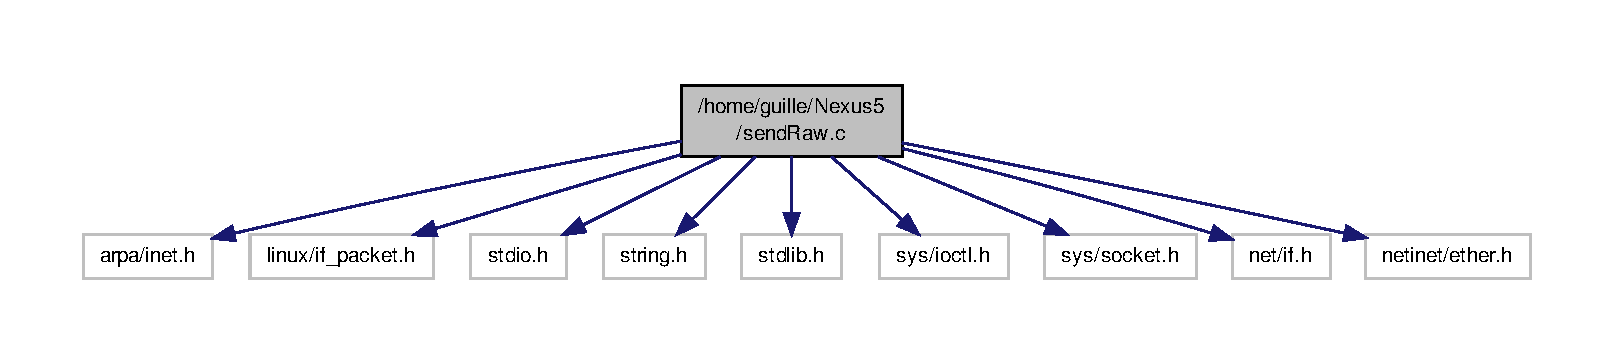
\includegraphics[width=350pt]{send_raw_8c__incl}
\end{center}
\end{figure}
\subsection*{Macros}
\begin{DoxyCompactItemize}
\item 
\#define \hyperlink{send_raw_8c_af68b987ceb49b8ac03521c2ac2b67466}{M\-Y\-\_\-\-D\-E\-S\-T\-\_\-\-M\-A\-C0}~0x00
\item 
\#define \hyperlink{send_raw_8c_abcb66f0a18511fdf5fb98ae7dc6a04c8}{M\-Y\-\_\-\-D\-E\-S\-T\-\_\-\-M\-A\-C1}~0x00
\item 
\#define \hyperlink{send_raw_8c_a55a86b2b53bbe0d3600a3e0d87d36fd5}{M\-Y\-\_\-\-D\-E\-S\-T\-\_\-\-M\-A\-C2}~0x00
\item 
\#define \hyperlink{send_raw_8c_ad987c3d374d7cf04c23f9ab884392606}{M\-Y\-\_\-\-D\-E\-S\-T\-\_\-\-M\-A\-C3}~0x00
\item 
\#define \hyperlink{send_raw_8c_a1faa80605f3bba48a4a5f9e249b080f3}{M\-Y\-\_\-\-D\-E\-S\-T\-\_\-\-M\-A\-C4}~0x00
\item 
\#define \hyperlink{send_raw_8c_a25c57a854ec54f333e002010d5f09981}{M\-Y\-\_\-\-D\-E\-S\-T\-\_\-\-M\-A\-C5}~0x00
\item 
\#define \hyperlink{send_raw_8c_aa09b857081f02c337190b7fd4e7096c4}{D\-E\-F\-A\-U\-L\-T\-\_\-\-I\-F}~\char`\"{}eth0\char`\"{}
\item 
\#define \hyperlink{send_raw_8c_a58958b9eb68ff960a6353298f9123738}{B\-U\-F\-\_\-\-S\-I\-Z}~1024
\end{DoxyCompactItemize}
\subsection*{Functions}
\begin{DoxyCompactItemize}
\item 
int \hyperlink{send_raw_8c_a0ddf1224851353fc92bfbff6f499fa97}{main} (int argc, char $\ast$argv\mbox{[}$\,$\mbox{]})
\end{DoxyCompactItemize}


\subsection{Macro Definition Documentation}
\hypertarget{send_raw_8c_a58958b9eb68ff960a6353298f9123738}{\index{send\-Raw.\-c@{send\-Raw.\-c}!B\-U\-F\-\_\-\-S\-I\-Z@{B\-U\-F\-\_\-\-S\-I\-Z}}
\index{B\-U\-F\-\_\-\-S\-I\-Z@{B\-U\-F\-\_\-\-S\-I\-Z}!sendRaw.c@{send\-Raw.\-c}}
\subsubsection[{B\-U\-F\-\_\-\-S\-I\-Z}]{\setlength{\rightskip}{0pt plus 5cm}\#define B\-U\-F\-\_\-\-S\-I\-Z~1024}}\label{send_raw_8c_a58958b9eb68ff960a6353298f9123738}
\hypertarget{send_raw_8c_aa09b857081f02c337190b7fd4e7096c4}{\index{send\-Raw.\-c@{send\-Raw.\-c}!D\-E\-F\-A\-U\-L\-T\-\_\-\-I\-F@{D\-E\-F\-A\-U\-L\-T\-\_\-\-I\-F}}
\index{D\-E\-F\-A\-U\-L\-T\-\_\-\-I\-F@{D\-E\-F\-A\-U\-L\-T\-\_\-\-I\-F}!sendRaw.c@{send\-Raw.\-c}}
\subsubsection[{D\-E\-F\-A\-U\-L\-T\-\_\-\-I\-F}]{\setlength{\rightskip}{0pt plus 5cm}\#define D\-E\-F\-A\-U\-L\-T\-\_\-\-I\-F~\char`\"{}eth0\char`\"{}}}\label{send_raw_8c_aa09b857081f02c337190b7fd4e7096c4}
\hypertarget{send_raw_8c_af68b987ceb49b8ac03521c2ac2b67466}{\index{send\-Raw.\-c@{send\-Raw.\-c}!M\-Y\-\_\-\-D\-E\-S\-T\-\_\-\-M\-A\-C0@{M\-Y\-\_\-\-D\-E\-S\-T\-\_\-\-M\-A\-C0}}
\index{M\-Y\-\_\-\-D\-E\-S\-T\-\_\-\-M\-A\-C0@{M\-Y\-\_\-\-D\-E\-S\-T\-\_\-\-M\-A\-C0}!sendRaw.c@{send\-Raw.\-c}}
\subsubsection[{M\-Y\-\_\-\-D\-E\-S\-T\-\_\-\-M\-A\-C0}]{\setlength{\rightskip}{0pt plus 5cm}\#define M\-Y\-\_\-\-D\-E\-S\-T\-\_\-\-M\-A\-C0~0x00}}\label{send_raw_8c_af68b987ceb49b8ac03521c2ac2b67466}
\hypertarget{send_raw_8c_abcb66f0a18511fdf5fb98ae7dc6a04c8}{\index{send\-Raw.\-c@{send\-Raw.\-c}!M\-Y\-\_\-\-D\-E\-S\-T\-\_\-\-M\-A\-C1@{M\-Y\-\_\-\-D\-E\-S\-T\-\_\-\-M\-A\-C1}}
\index{M\-Y\-\_\-\-D\-E\-S\-T\-\_\-\-M\-A\-C1@{M\-Y\-\_\-\-D\-E\-S\-T\-\_\-\-M\-A\-C1}!sendRaw.c@{send\-Raw.\-c}}
\subsubsection[{M\-Y\-\_\-\-D\-E\-S\-T\-\_\-\-M\-A\-C1}]{\setlength{\rightskip}{0pt plus 5cm}\#define M\-Y\-\_\-\-D\-E\-S\-T\-\_\-\-M\-A\-C1~0x00}}\label{send_raw_8c_abcb66f0a18511fdf5fb98ae7dc6a04c8}
\hypertarget{send_raw_8c_a55a86b2b53bbe0d3600a3e0d87d36fd5}{\index{send\-Raw.\-c@{send\-Raw.\-c}!M\-Y\-\_\-\-D\-E\-S\-T\-\_\-\-M\-A\-C2@{M\-Y\-\_\-\-D\-E\-S\-T\-\_\-\-M\-A\-C2}}
\index{M\-Y\-\_\-\-D\-E\-S\-T\-\_\-\-M\-A\-C2@{M\-Y\-\_\-\-D\-E\-S\-T\-\_\-\-M\-A\-C2}!sendRaw.c@{send\-Raw.\-c}}
\subsubsection[{M\-Y\-\_\-\-D\-E\-S\-T\-\_\-\-M\-A\-C2}]{\setlength{\rightskip}{0pt plus 5cm}\#define M\-Y\-\_\-\-D\-E\-S\-T\-\_\-\-M\-A\-C2~0x00}}\label{send_raw_8c_a55a86b2b53bbe0d3600a3e0d87d36fd5}
\hypertarget{send_raw_8c_ad987c3d374d7cf04c23f9ab884392606}{\index{send\-Raw.\-c@{send\-Raw.\-c}!M\-Y\-\_\-\-D\-E\-S\-T\-\_\-\-M\-A\-C3@{M\-Y\-\_\-\-D\-E\-S\-T\-\_\-\-M\-A\-C3}}
\index{M\-Y\-\_\-\-D\-E\-S\-T\-\_\-\-M\-A\-C3@{M\-Y\-\_\-\-D\-E\-S\-T\-\_\-\-M\-A\-C3}!sendRaw.c@{send\-Raw.\-c}}
\subsubsection[{M\-Y\-\_\-\-D\-E\-S\-T\-\_\-\-M\-A\-C3}]{\setlength{\rightskip}{0pt plus 5cm}\#define M\-Y\-\_\-\-D\-E\-S\-T\-\_\-\-M\-A\-C3~0x00}}\label{send_raw_8c_ad987c3d374d7cf04c23f9ab884392606}
\hypertarget{send_raw_8c_a1faa80605f3bba48a4a5f9e249b080f3}{\index{send\-Raw.\-c@{send\-Raw.\-c}!M\-Y\-\_\-\-D\-E\-S\-T\-\_\-\-M\-A\-C4@{M\-Y\-\_\-\-D\-E\-S\-T\-\_\-\-M\-A\-C4}}
\index{M\-Y\-\_\-\-D\-E\-S\-T\-\_\-\-M\-A\-C4@{M\-Y\-\_\-\-D\-E\-S\-T\-\_\-\-M\-A\-C4}!sendRaw.c@{send\-Raw.\-c}}
\subsubsection[{M\-Y\-\_\-\-D\-E\-S\-T\-\_\-\-M\-A\-C4}]{\setlength{\rightskip}{0pt plus 5cm}\#define M\-Y\-\_\-\-D\-E\-S\-T\-\_\-\-M\-A\-C4~0x00}}\label{send_raw_8c_a1faa80605f3bba48a4a5f9e249b080f3}
\hypertarget{send_raw_8c_a25c57a854ec54f333e002010d5f09981}{\index{send\-Raw.\-c@{send\-Raw.\-c}!M\-Y\-\_\-\-D\-E\-S\-T\-\_\-\-M\-A\-C5@{M\-Y\-\_\-\-D\-E\-S\-T\-\_\-\-M\-A\-C5}}
\index{M\-Y\-\_\-\-D\-E\-S\-T\-\_\-\-M\-A\-C5@{M\-Y\-\_\-\-D\-E\-S\-T\-\_\-\-M\-A\-C5}!sendRaw.c@{send\-Raw.\-c}}
\subsubsection[{M\-Y\-\_\-\-D\-E\-S\-T\-\_\-\-M\-A\-C5}]{\setlength{\rightskip}{0pt plus 5cm}\#define M\-Y\-\_\-\-D\-E\-S\-T\-\_\-\-M\-A\-C5~0x00}}\label{send_raw_8c_a25c57a854ec54f333e002010d5f09981}


\subsection{Function Documentation}
\hypertarget{send_raw_8c_a0ddf1224851353fc92bfbff6f499fa97}{\index{send\-Raw.\-c@{send\-Raw.\-c}!main@{main}}
\index{main@{main}!sendRaw.c@{send\-Raw.\-c}}
\subsubsection[{main}]{\setlength{\rightskip}{0pt plus 5cm}int main (
\begin{DoxyParamCaption}
\item[{int}]{argc, }
\item[{char $\ast$}]{argv\mbox{[}$\,$\mbox{]}}
\end{DoxyParamCaption}
)}}\label{send_raw_8c_a0ddf1224851353fc92bfbff6f499fa97}

%--- End generated contents ---

% Index
\newpage
\phantomsection
\addcontentsline{toc}{part}{Index}
\printindex

\end{document}
